\documentclass[12pt]{beamer}
\usetheme{Penn} 
\usepackage{amsmath, amssymb, amsthm, amsfonts}
\usepackage{graphicx}
\usepackage{fancyvrb}
\usepackage{verbatim}
%\usepackage{tabularx}
\usepackage{tikz}
\usepackage{animate}
\usetikzlibrary{matrix, shapes, arrows, calc, backgrounds}
\usepackage[vcentermath, enableskew]{youngtab}
\newcommand{\ZZ}{\ensuremath{\mathbb{Z}}}
\newcommand{\RR}{\ensuremath{\mathbb{R}}}
\newcommand{\PP}{\ensuremath{\mathbb{P}}}

\newcommand{\CC}{\ensuremath{\mathbb{C}}}

\newtheorem{thm}{Theorem}[section]
\newtheorem{cor}[thm]{Corollary}
\newtheorem{lem}[thm]{Lemma}
\newtheorem{prop}[thm]{Proposition}
\theoremstyle{definition}
\newtheorem{conj}[thm]{Conjecture}
\newtheorem{defn}[thm]{Definition}
\newtheorem{ex}[thm]{Example}
\newtheorem{rmk}[thm]{Remark}
\newtheorem{alg}[thm]{Algorithm}
\newtheorem{question}[thm]{Question}
\begin{document}

\author[Z. Rosen]{Zvi Rosen \\ Department of Mathematics}

\date[\today]{\today}
\title[Gauss Elimination]{{\Large Gauss Elimination}}
\institute[Dept. of Mathematics~~--~~University of Pennsylvania]{}


\frame{\titlepage}


\begin{frame}
\frametitle{Guiding Question}

Given a matrix equation $Ax = b$, for a real matrix $A$ and a
real vector $b$, how do we find a solution $x$?
\end{frame}
\begin{frame}
\frametitle{Graphical Method}

Consider each equation as defining a line / plane / hyperplane
in Euclidean space.

\vspace{1cm}
Draw each plane and see where they all intersect.
\end{frame}

\begin{frame}
\frametitle{Cramer's Rule}

For $Ax = b$, let $A_j =$ the matrix formed by replacing
the $j$-th column of $A$ with $b$. Then:

\[ x_j = \frac{\operatorname{det}(A_j)}{\operatorname{det}(A)}.\]

What is the determinant of a matrix? See next slide.
\end{frame}

\begin{frame}
\frametitle{Determinants}

The determinant of a square matrix $A$ can be defined inductively
as follows:
\begin{enumerate}
\item The determinant of a $1 \times 1$ matrix is its only entry.
\item The determinant of a $n \times n$ matrix can be obtained by:
Fixing a row $j$. Defining the matrix $A({j,k})$ to be the matrix
leaving out the $j$-th row and $k$-th column. 
\[ \det(A) = \sum_{k = 1}^n (-1)^{j+k}A_{j,k}\det(A(j,k))
\]

\end{enumerate}
\end{frame}

\begin{frame}
\frametitle{Determinants -- Geometric View}
If you consider the matrix $A$ as a linear map between
two vector spaces, then the determinant can be thought of
as the volume of the unit cube after passing through
the map $A$.

\centerline{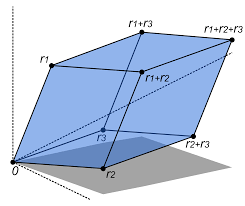
\includegraphics[scale = .6]{gauss1.png}}

\flushright{\tiny --image from Wikipedia.}

\end{frame}

\begin{frame}
\frametitle{Naive Gauss Elimination}
INPUT: $n \times (n+1)$ Matrix $A|b$
\begin{enumerate}
\item Fix pivot variable $A_{1,1}$.
\item Perform {\bf row operations} to eliminate everything 
below the pivot variable.
\item If $k < n$, change pivot variable from $A_{k,k}$ to $A_{k+1,k+1}$
and repeat step 2.
\item Solve for $x_k$ and substitute its value into Row $k-1$. Repeat to
solve for each $x_k$.
\end{enumerate}
Row operations: Permute rows, add a scalar multiple of row $j$
to row $k$.
\end{frame}

\begin{frame}
\frametitle{Naive Gaussian Elimination - Example}

\[
\left(\begin{array}{ccc|c}
1 & 2 & 3 & 4 \\
6 & 5 & 8 & 7 \\
3 & 1 & 4 & 2 \\
\end{array}\right)\]
\end{frame}

\begin{frame}
\frametitle{Naive Gauss - Complexity}
How many operations does Naive Gaussian elimination take?

\begin{align*}
\# \text{operations} =& \sum_{k = 1}^{n-1} \# (\text{operations at pivot  } k)\\
+& \sum_{k=1}^{n} \#(\text{operations to solve for  } x_k) \\
=& \sum_{k = 1}^{n-1} 2(n-k)(n-k-1) + \sum_{k = 1}^{n} (n-k + 2)
\end{align*}
\end{frame}


\begin{frame}
\frametitle{Naive Gauss - Complexity}
\begin{align*}
=& \sum_{k=1}^{n-1} 2n^2 - \sum_{k=1}^{n-1}4nk +  \sum_{k=1}^{n-1}2 k^2 - \sum_{k=1}^{n-1} 2n \\
+& \sum_{k=1}^{n-1} 2k + \sum_{k = 1}^n n - \sum_{k=1}^{n} k + \sum_{k=1}^n 2.\\
=& 2n^3 - 3n^2 + 3n + (-4n+1)\sum_{k=1}^{n-1} k + 2\sum_{k=1}^{n-1} k^2.
\end{align*}
Note that $\sum_{k=1}^{n-1} k = \frac{1}{2} n^2 + O(n)$ and 
 $\sum_{k=1}^{n-1} k^2 = \frac{1}{3} n^3 + O(n^2)$.
\end{frame}


\begin{frame}
\frametitle{Naive Gauss - Complexity}

So we are left with: 
\begin{align*}
=& 2n^3 - 3n^2 + 3n + (-4n+1)(\frac{1}{2} n^2 + O(n)) + 2(\frac{1}{3}n^3 + O(n^2))\\
=& \frac{2}{3}n^3 + O(n^2).
\end{align*}
\end{frame}

\begin{frame}
\frametitle{Pivoting}
We have to be careful! Sometimes $A_{k,k} = 0$ or is
numerically very close to zero.
\begin{itemize}
\item Partial pivoting means at each step, search column $k$ for
the largest element $A_{jk}$ then switch rows $j$ and $k$.
\item Complete pivoting means that we also search for the highest
value in the row $j$ (This would mean relabeling variables, which is
undesirable).
\end{itemize}
\end{frame}

\begin{frame}
\frametitle{Pivoting - Example}

\begin{ex}
$$\left(\begin{array}{cc}
.0003 & 3.0000  \\
1.0000 & 1.0000  \\
\end{array}\right)
\left(\begin{array}{c}
x_1  \\
x_2 \\
\end{array}\right) = 
\left(\begin{array}{c}
2.0001  \\
1.0000 \\
\end{array}\right)$$
\end{ex}
Compare the results you obtain via naive Gaussian elimination,
and pivoting. (Use MATLAB for your computation.)



\end{frame}

\begin{frame}
\frametitle{Tridiagonal Systems}
A tridiagonal system is a matrix equation $Ax = b$,
when the only nonzero entries of $A$ are $A_{i,i-1}, A_{i,i}$,
and $A_{i,i+1}$ (wherever these indices make sense).

\[
\left(\begin{array}{cccccc}
a_{1,1} & a_{1,2} & 0 & 0 & \cdots & 0 \\
a_{2,1} & a_{2,2} & a_{2,3} & 0 & \cdots & 0 \\[3mm]
0 & \ddots & \ddots & \ddots & &\vdots \\[3mm]
0  & \cdots & \cdots & 0 & a_{n-1,n} & a_{n,n}  \\
\end{array}\right)
\]
\end{frame}

\begin{frame}
\frametitle{Tridiagonal Systems - Complexity}

{\bf Question:} How many operations does Gaussian Elimination take
for a tridiagonal system?

\vspace{1cm}

Perform a complexity computation similar to the slides
above regarding Naive Gaussian Elimination, accounting for
both elimination and substitution steps. Your result should
be $O(n)$.
\end{frame}

\begin{frame}
\frametitle{LU Factorization}
{\bf Problem:} Find a way to quickly solve $Ax = b$ when $A$ is fixed
but we want to solve for a number of inputs $b$.

\vspace{1cm} 

{\bf Idea:} Factor $A$ as $A = LU$ where $L$ is lower-triangular
and $U$ is upper-triangular. Then, suppose there exists a vector $d$
so that $Ld = b$.
\[ Ax = b \implies LUx = b \implies LUx = Ld \iff Ux = d.\]
At this point, we have two equations with triangular matrices:
\[ Ux = d, Ld = b.\]

\end{frame}

\begin{frame}
\frametitle{Solving with LU Factorization}
Given these two triangular systems $Ux = d, Ld = b$, we
do not need to worry about the elimination part of Gaussian elimination
-- just the substitution part. 

\vspace{5mm}

Solve for $d_1$ through $d_n$ substituting down at each step.\\
Then solve for $x_n$ through $x_1$ substituting up at each step.\\
This drastically cuts down complexity.
\end{frame}

\begin{frame}
\frametitle{LU Factorization -- How?}
It should be clear by now that an LU factorization
would be really useful for equation solving. But how
do we obtain it? Fix $A$ as our matrix.

Perform the standard Gaussian elimination, when our pivot 
variable is $A_{kk}$, we eliminate
entry $A_{jk}$ below the diagonal by replacing row $R_j$ with $c_{jk}*R_k + R_j$.
Set $L_{jk}$ to be $-c_{jk}$.

\begin{itemize}
\item $U$ is the matrix spit out by Gaussian elimination.
\item $L$ is the matrix with ones on the diagonal, and the lower entries
obtained as above.
\end{itemize}
\end{frame}

\begin{frame}
\frametitle{LU Factorization - Example}

Let $A$ be the matrix:

\[
\left(\begin{array}{ccc}
1 & 2 & 3  \\
6 & 5 & 8  \\
3 & 1 & 4  \\
\end{array}\right)\]

Let $b$ be the vector $(4,7,2)$. Solve $Ax = b$ by:
\begin{enumerate}
\item Standard Gaussian Elimination.
\item Finding $A = LU$ then solving $Ld = b$ and $Ux = d$.
\end{enumerate}
\end{frame}
\end{document}
